% /**
%  * A template for homework files in math classes. The 
%  * packages and newcommands are a good starting point.
%  *
%  * Author: James K. Pringle
%  * E-mail: jameskpringle@gmail.com
%  * Last Changed: 5 September 2013
%  *
%  * "LaTeX countains the increasing union of MS Word"
%  */
%~~~~~~~~~~~~~~~~~~~~~~~~~~~~~~~~~~~~~~~~~~~~~~~~~~~~~~~~~%
%%%%%%%%%%%%%%%%%%%%%%%%%%%%%%%%%%%%%%%%%%%%%%%%%%%%%%%%%%%
%                                                         %
%                        PAGE SETUP                       %
%                                                         %
%%%%%%%%%%%%%%%%%%%%%%%%%%%%%%%%%%%%%%%%%%%%%%%%%%%%%%%%%%%
\documentclass[letterpaper, 12pt]{article}\usepackage[]{graphicx}\usepackage[]{color}
%% maxwidth is the original width if it is less than linewidth
%% otherwise use linewidth (to make sure the graphics do not exceed the margin)
\makeatletter
\def\maxwidth{ %
  \ifdim\Gin@nat@width>\linewidth
    \linewidth
  \else
    \Gin@nat@width
  \fi
}
\makeatother

\definecolor{fgcolor}{rgb}{0.345, 0.345, 0.345}
\newcommand{\hlnum}[1]{\textcolor[rgb]{0.686,0.059,0.569}{#1}}%
\newcommand{\hlstr}[1]{\textcolor[rgb]{0.192,0.494,0.8}{#1}}%
\newcommand{\hlcom}[1]{\textcolor[rgb]{0.678,0.584,0.686}{\textit{#1}}}%
\newcommand{\hlopt}[1]{\textcolor[rgb]{0,0,0}{#1}}%
\newcommand{\hlstd}[1]{\textcolor[rgb]{0.345,0.345,0.345}{#1}}%
\newcommand{\hlkwa}[1]{\textcolor[rgb]{0.161,0.373,0.58}{\textbf{#1}}}%
\newcommand{\hlkwb}[1]{\textcolor[rgb]{0.69,0.353,0.396}{#1}}%
\newcommand{\hlkwc}[1]{\textcolor[rgb]{0.333,0.667,0.333}{#1}}%
\newcommand{\hlkwd}[1]{\textcolor[rgb]{0.737,0.353,0.396}{\textbf{#1}}}%

\usepackage{framed}
\makeatletter
\newenvironment{kframe}{%
 \def\at@end@of@kframe{}%
 \ifinner\ifhmode%
  \def\at@end@of@kframe{\end{minipage}}%
  \begin{minipage}{\columnwidth}%
 \fi\fi%
 \def\FrameCommand##1{\hskip\@totalleftmargin \hskip-\fboxsep
 \colorbox{shadecolor}{##1}\hskip-\fboxsep
     % There is no \\@totalrightmargin, so:
     \hskip-\linewidth \hskip-\@totalleftmargin \hskip\columnwidth}%
 \MakeFramed {\advance\hsize-\width
   \@totalleftmargin\z@ \linewidth\hsize
   \@setminipage}}%
 {\par\unskip\endMakeFramed%
 \at@end@of@kframe}
\makeatother

\definecolor{shadecolor}{rgb}{.97, .97, .97}
\definecolor{messagecolor}{rgb}{0, 0, 0}
\definecolor{warningcolor}{rgb}{1, 0, 1}
\definecolor{errorcolor}{rgb}{1, 0, 0}
\newenvironment{knitrout}{}{} % an empty environment to be redefined in TeX

\usepackage{alltt}

% 1in margins all the way around
\usepackage[margin=1in]{geometry}

% Sets \parindent to 0 and \parskip to stretchable.
\usepackage{parskip}
% Use for bigger spaces between paragraphs.
%\parskip=1.5\baselineskip

% Set headers and footers
\usepackage{fancyhdr}
\pagestyle{fancy}
% Header
\renewcommand{\headrulewidth}{0.4pt}
\lhead{\textsc{\mathclass}}
\chead{\textsc{\today}}
\rhead{\textsc{\mynamehdr}}
% Footer
\renewcommand{\footrulewidth}{0.4pt}
\lfoot{}
\cfoot{\thepage}
\rfoot{}

% Make the space between lines slightly more generous 
% than normal single spacing, but compensate so that the 
% spacing between rows of matrices still looks normal.  
% Note that 1.1=1/.9090909...
\renewcommand{\baselinestretch}{1.1}
\renewcommand{\arraystretch}{.91}

%%%%%%%%%%%%%%%%%%%%%%%%%%%%%%%%%%%%%%%%%%%%%%%%%%%%%%%%%%%
%                                                         %
%                      USEFUL PACKAGES                    %
%                                                         %
%%%%%%%%%%%%%%%%%%%%%%%%%%%%%%%%%%%%%%%%%%%%%%%%%%%%%%%%%%%

% The classic three
\usepackage{amsmath,amsthm,amssymb}

% Define \newtheorem for use
% No numbers, labeled 'Theorem'
\newtheorem*{nthm}{Theorem}

% Not sure what this is for
\usepackage{amsfonts}

% Fancy script font
\usepackage{mathrsfs}

% Makes enumerate environment much easier to customize
% by specifying the counter
\usepackage{enumerate}

% Color
\usepackage{color}
\usepackage[usenames,dvipsnames,svgnames,table]{xcolor}

% URL links
\usepackage{hyperref}

% For inserting graphics and images
\usepackage{graphicx}
\usepackage{float}
\usepackage[footnotesize]{caption}



%%%%%%%%%%%%%%%%%%%%%%%%%%%%%%%%%%%%%%%%%%%%%%%%%%%%%%%%%%%
%                                                         %
%                   USER-DEFINED COMMANDS                 %
%                                                         %
%%%%%%%%%%%%%%%%%%%%%%%%%%%%%%%%%%%%%%%%%%%%%%%%%%%%%%%%%%%

% Make a hyperlink with colored text
\newcommand{\hrefcolor}[3]{\href{#1}{\textcolor{#3}{#2}}}

% Make a hyperlink with gray text
\newcommand{\hrefgray}[2]{\hrefcolor{#1}{#2}{Gray}}

% Make the header for the first page
\newcommand{\firstpageinfo}{
\textsf{
\begin{flushleft}
\sc \myname \\
\normalfont \mathclass \\
\professorname \\
\assignmentnumber \\
\thedate
\end{flushleft}
} \bigskip
}

% Make problem list for "title" of page
\newcommand{\problemlist}{ 
\begin{center}
\textbf{\Large \textsf{\assignmentnumber}}\\
\textit{\textsf{\problemset}}
\end{center}
\bigskip
}

%~~~~~~~~~~~~~~~~~~~~~~~~~~~~~~~~~~~~~~~~~~~~~~~~~~~~~~~~~%
%                                                         %
%               LETTERS, FUNCTIONS, AND TEXT              %
%                                                         %
%~~~~~~~~~~~~~~~~~~~~~~~~~~~~~~~~~~~~~~~~~~~~~~~~~~~~~~~~~%

% A
\newcommand{\cA}{\mathcal{A}}
\newcommand{\sA}{\mathscr{A}}
\renewcommand{\aa}{\;\text{a.a.}}
\renewcommand{\ae}{\;\text{a.e.}}
% B
\newcommand{\B}{\mathscr{B}}
\newcommand{\cB}{\mathcal{B}}
% C
\newcommand{\cC}{\mathcal{C}}
\newcommand{\cov}{\text{cov}}
% E
\newcommand{\E}{\mathbb{E}}
% F
\newcommand{\sF}{\mathscr{F}}
\newcommand{\cF}{\mathcal{F}}
\newcommand{\Ft}{F^\sim}
% G
\newcommand{\cG}{\mathcal{G}}
\newcommand{\sG}{\mathscr{G}}
% I
\newcommand{\io}{\;\text{i.o.}}
% N
\newcommand{\N}{\mathbb{N}}
% P
\newcommand{\cP}{\mathcal{P}}
\newcommand{\sP}{\mathscr{P}}
\newcommand{\pr}{\text{pr}}
% Q
\newcommand{\Q}{\mathbb{Q}}
% R
\newcommand{\R}{\mathbb{R}}
\newcommand{\bR}{\mathbf{R}}
\newcommand{\cR}{\mathcal{R}}
% S
\newcommand{\cS}{\mathcal{S}}
% U
\newcommand{\cU}{\mathcal{U}}
% V
\newcommand{\var}{\text{var}}
% Z
\newcommand{\Z}{\mathbb{Z}}
% Punctuation
\newcommand{\sbs}{\;|\;} % space bar space
% Math
\newcommand{\imii}{\int_{-\infty}^\infty}
\newcommand{\pion}{\prod_{i=1}^n}
\newcommand{\pioI}{\prod_{i=1}^I}
\newcommand{\pjon}{\prod_{j=1}^n}
\newcommand{\pjoJ}{\prod_{j=1}^J}
\newcommand{\pkon}{\prod_{k=1}^n}
\newcommand{\pkoK}{\prod_{k=1}^K}
\newcommand{\sion}{\sum_{i=1}^n}
\newcommand{\sioI}{\sum_{i=1}^I}
\newcommand{\sjon}{\sum_{j=1}^n}
\newcommand{\sjoJ}{\sum_{j=1}^J}
\newcommand{\skon}{\sum_{k=1}^n}
\newcommand{\skoK}{\sum_{k=1}^K}
\newcommand{\sioi}{\sum_{i=1}^\infty}
\newcommand{\sjoi}{\sum_{j=1}^\infty}
\newcommand{\skoi}{\sum_{k=1}^\infty}
\newcommand{\sio}{\sum_{i=1}}
\newcommand{\sjo}{\sum_{j=1}}
\newcommand{\sko}{\sum_{k=1}}
% Typography
\newcommand{\scb}[1]{\textsc{\textbf{#1}}}

%~~~~~~~~~~~~~~~~~~~~~~~~~~~~~~~~~~~~~~~~~~~~~~~~~~~~~~~~~%
%                                                         %
%            CHANGE THESE BASED ON THE PAPER              %
%                                                         %
%~~~~~~~~~~~~~~~~~~~~~~~~~~~~~~~~~~~~~~~~~~~~~~~~~~~~~~~~~%

% Constants for fancy header and first page info
\newcommand{\mynamehdr}{\hrefgray{http://biostat.jhsph.edu/~jpringle/}{\myname}}
\newcommand{\mathclass}{140.673 Theory}
\newcommand{\myname}{James K. Pringle}
\newcommand{\professorname}{Dr. Constantine Frangakis}
\newcommand{\assignmentnumber}{Assignment 4}
\newcommand{\thedate}{\today}
\newcommand{\problemset}{}

%%%%%%%%%%%%%%%%%%%%%%%%%%%%%%%%%%%%%%%%%%%%%%%%%%%%%%%%%%%
%                                                         %
%                      BEGIN DOCUMENT                     %
%                                                         %
%%%%%%%%%%%%%%%%%%%%%%%%%%%%%%%%%%%%%%%%%%%%%%%%%%%%%%%%%%%
\IfFileExists{upquote.sty}{\usepackage{upquote}}{}
\begin{document}

% Take header off of first page
\thispagestyle{empty}

% Put in first page info (top of page)
\firstpageinfo

% Put in title for the paper
\problemlist


%%%%%%%%%%%%%%%%%%%%%%%%%%%%%%%%%%%%%%%%%%%%%%%%%%%%%%%%%%%
%                                                         %
%                     Start Problem 1                     %
%                                                         %
%%%%%%%%%%%%%%%%%%%%%%%%%%%%%%%%%%%%%%%%%%%%%%%%%%%%%%%%%%%
\subsection*{Problem 1}
\begin{enumerate}[(a)]
\item
Are the following families of distributions exponential families?

\begin{proof}
The Gamma$(a,b)$ is in the exponential family. Its density is 
\[
\frac{b^a}{\Gamma(a)} x^{a - 1} e^{-bx} = 
\frac{b^a}{\Gamma(a)}
\exp\left\{
-bx +(a-1)\log(x)
\right\}
=
\frac{b^a}{\Gamma(a)} \exp\left\{ \begin{bmatrix}
a - 1 & -b
\end{bmatrix}
\begin{bmatrix}
\log x \\
x
\end{bmatrix} 
\right\}
\]
By chapter 4, slide 2, of the course notes, since the Gamma$(a,b)$ can be written as 
\[
f_{\mathbf{X}} (\mathbf{x}; \boldsymbol{\theta})
=
c(\boldsymbol{\theta})
h(\mathbf{x})
\exp
\left\{
\sum_{j=1}^k
\gamma_j(\boldsymbol{\theta})
t_j(\mathbf{x})
\right\}
\]
the Gamma$(a,b)$ is a member of the exponential family of distributions.

The Weibull$(c,d)$ is not an exponential family because there is a term in the exponential with both data and parameters that cannot be separated into a function of the data multiplied by a function of the parameters. Suppose $\theta = (c,d)$. There are no functions $w(\theta)$ and $f(t)$ such that 
\[
w(\theta)f(t) = -dt^c
\]
\end{proof}

\item
When using only the theorem discussed in class for judging completeness of the minimal sufficient statistics (MSS), can we deduce that the MSS for the parameters based on an i.i.d. sample from the families below is complete?
\begin{enumerate}[(i)]
\item
Gamma$(a,b), a>0, b>0,$ where the mean is $a/b$ and the variance is $a/b^2$.

\begin{proof}
For the Gamma$(a,b)$, the natural parameter space is 
\[
\{
(a-1, -b) : a, b > 0
\}
\]
This contains a rectangle, for example
\[
\{
(a,b) : 1 \leq a \leq 2, -1 \leq b \leq -2
\}
\]
According to the theorem, found on Lecture 4, slide 4, the MSS is also complete.
\end{proof}

\item
The Weibull$(c,d)$ distributions, whose density at $t>0$ is
\[
f(t|c,d) = cdt^{c-1}\exp(-dt^c), \text{ for }c>0, d>0
\]

\begin{proof}
Since the Weibull is as given, with $c$ allowed to vary, it is not in the exponential family. Therefore, the theorem discussed in class cannot be applied to it.
\end{proof}
\end{enumerate}
\end{enumerate}

\subsection*{Problem 2. Cramer Rao bounds with multiple parameters.}
(Before you start answering the first question, read all of the questions and the final note carefully).

We want to study the length of time $T$ that a special type of cells spends during DNA synthesis. Assume
that we can conduct a study where we can observe the actual times $T_i$ of an i.i.d. sample $i = 1, \dots, n$ from
the population of cells. Assume also that in the population of cells, the times (measured in hours) have
approximately the Weibull distribution, given in part (ii) above, for some unknown true parameter values
$c_0$, $d_0$.

\begin{enumerate}[(i)]
\item
Find expressions for the scores for $c$ and $d$ defined, respectively, as:
\[
S_{i, c_0} = 
\frac{\partial \log f(t|c,d)}{\partial c}
|
_{t=T_i, c=c_0, d=d_0},
\text{ and }
S_{i, d_0} =
\frac{\partial \log f(t|c,d)}{\partial d}
|
_{t=T_i, c=c_0, d=d_0}
\]

\begin{proof}
Note
\[
\log f(t|c,d) = \log [cdt^{c-1}\exp(-dt^c)]
= \log c + \log d + (c-1) \log t - dt^c
\]
Hence
\[
S_{i, c_0} = 
\frac{\partial \log f(t|c,d)}{\partial c}
|
_{t=T_i, c=c_0, d=d_0}
=
1/c_0 + \log T_i - d_0 T_i^{c_0} \log T_i
\]
and
\[
S_{i, d_0} = 
\frac{\partial \log f(t|c,d)}{\partial d}
|
_{t=T_i, c=c_0, d=d_0}
=
1/d_0 - T_i^c
\]
\end{proof}

\item
By noting that
$\partial(t^c) / \partial(t) = ct^{c-1}$, show that the cumulative distribution function $\pr(T<t | c,d) = 1 - \exp(-dt^c)$. Hence, or otherwise, describe explicitly how you can simulate a random sample of 100000 lengths of time from the Weibull if you knew $c_0, d_0$.
\begin{proof}
Since the Weibull is defined on non-negative real numbers, $\pr(T<t |c,d) = 0$ for $t < 0$.
Notice
\[
\lim_{t \to \infty}
\pr(T<t | c,d)
=
1 - 0 = 1
\]
and 
\[
\lim_{t \to 0}
\pr(T<t | c,d)
=
1- 1
=
0
\]
Furthermore, $\pr(T<t | c,d)$ is continuous in $t$ (hence right-continuous) because it is a composition of continuous functions. If $0 \leq t_1 \leq t_2$, then
\begin{align*}
-dt_1^c &\geq -dt_2^c \\
1-\exp(-dt_1^c) &\leq 1 -\exp(-dt_2^c)
\end{align*}
so that $\pr(T<t | c,d)$ is increasing. Therefore $\pr(T<t | c,d)$ is a distribution function.

Calculating,
\[
\frac{d \; \pr(T<t | c,d)}{dt}
=
\frac{d}{dt}
(1 - \exp(-dt^c))
=
dct^{c-1} \exp(-dt^c)
\]
The derivative of the distribution function is the Weibull density with parameters $c$ and $d$. Hence, $\pr(T<t | c,d)$ is the distribution function of the Weibull$(c,d)$. 

Let $F(t|c,d) = \pr(T<t | c,d)$. The inverse distribution function is 
\begin{align*}
F^{-1}(y|c,d) = \left(\frac{-\log (1-y)}{d} \right)^{1/c}
\end{align*}
since
\begin{align*}
F(F^{-1}(y|c,d)) 
&= 1 - \exp
\left(
-d 
\left(
\left(\frac{-\log (1-y)}{d} \right)^{1/c}
\right) ^c
\right)
\\
&=
1 - \exp(\log(1-y))
\\
&=
y
\end{align*}
and similarly $F^{-1}(F(t|c,d)) = t$. By a well-known result, if $U \sim Uniform(0,1)$, then 
\[
\pr(F^{-1}(U|c,d) < t) = \pr(T < t |c,d)  = F(t|c,d) 
\]
Hence, to similuate Weibull$(c,d)$, it is sufficient to draw a uniform on $(0,1)$, then to apply $F^{-1}$ to that random draw. This of course can be done 100,000 times.

\begin{knitrout}
\definecolor{shadecolor}{rgb}{0.969, 0.969, 0.969}\color{fgcolor}\begin{kframe}
\begin{alltt}
\hlstd{rwei} \hlkwb{<-} \hlkwa{function}\hlstd{(}\hlkwc{n}\hlstd{,} \hlkwc{c}\hlstd{,} \hlkwc{d}\hlstd{) \{}
    \hlstd{u} \hlkwb{<-} \hlkwd{runif}\hlstd{(n)}
    \hlstd{(}\hlopt{-}\hlkwd{log}\hlstd{(}\hlnum{1} \hlopt{-} \hlstd{u)}\hlopt{/}\hlstd{d)}\hlopt{^}\hlstd{(}\hlnum{1}\hlopt{/}\hlstd{c)}
\hlstd{\}}

\hlstd{k} \hlkwb{<-} \hlnum{1e+05}
\hlstd{c} \hlkwb{<-} \hlnum{3}
\hlstd{d} \hlkwb{<-} \hlnum{0.002}

\hlstd{x} \hlkwb{<-} \hlkwd{rwei}\hlstd{(k, c, d)}

\hlkwd{summary}\hlstd{(x)}
\end{alltt}
\begin{verbatim}
##    Min. 1st Qu.  Median    Mean 3rd Qu.    Max. 
##   0.133   5.250   7.030   7.090   8.860  19.800
\end{verbatim}
\begin{alltt}
\hlkwd{plot}\hlstd{(}\hlkwd{density}\hlstd{(x),} \hlkwc{main} \hlstd{=} \hlstr{"Density of simulated Weibull(3, 0.002)"}\hlstd{)}
\end{alltt}
\end{kframe}
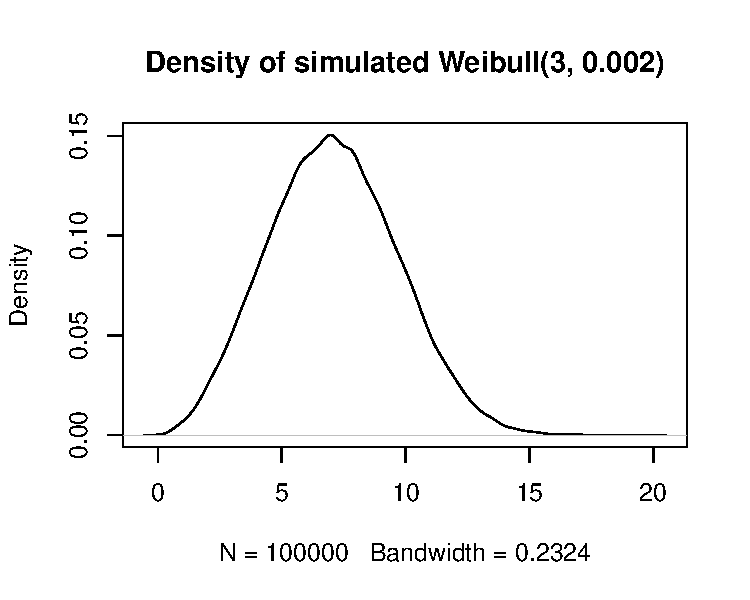
\includegraphics[width=\maxwidth]{figure/rwei} 

\end{knitrout}

\end{proof}

\item
Suppose Dr. Fin, the lab’s researcher, knows only that $d_0 = .002$, and Dr. Fin wants to use the data $T_i$,
$i = 1, \dots, n$ to estimate $c_0$. Find the Cramer-Rao bound (CRb) for \underline{Dr. Fin’s estimation} of $c_0$, if \underline{we} also
know that $c_0 = 3$. (Note: the only unknown in your result should be the sample size $n$). (Hint: use the
relation between scores and the CRb, also, because the analytic (i.e. closed form) calculation of CRb
here is difficult, you may want to use a method that is not analytic, if you do, describe the method.)

\begin{proof}
Since $c$ is the only parameter that defines the distribution, the Fisher information of a single observation is
\[
I_1(c_0) = E(S_{i,c_0}^2 | c_0)
\]
Since the data are i.i.d. (assuming there are $n$ data points) the CRb for a unbiased estimator of $c_0$, under regularity conditions, is
\[
(nI_1(c_0))^{-1}
\]
by course slides chapter 5, slide 2.
Since the expression for $S_{i,c_0}^2$ is complicated, we approximate its expectation numerically. According to the Law of Large Numbers, 
\[
\widehat{I_k(c_0)} = 
\frac{1}{k} \sum_{i=1}^k S_{i,c_0}^2 \to E(S_{i,c_0}^2 | c_0) = I_1(c_0)
\]
where $\{S_{i,c_0}^2\}_{i \geq 1}$ represents a sequence of realized random variables. 
Therefore, for $k$ large, we use $k$ simulated Weibull$(c_0,d_0)$, where $c_0 = 3$ and $d_0 = 0.002$, to get an approximation of $I_1(c_0)$.

\begin{knitrout}
\definecolor{shadecolor}{rgb}{0.969, 0.969, 0.969}\color{fgcolor}\begin{kframe}
\begin{alltt}
\hlstd{score_c} \hlkwb{<-} \hlkwa{function}\hlstd{(}\hlkwc{x}\hlstd{,} \hlkwc{c}\hlstd{,} \hlkwc{d}\hlstd{) \{}
    \hlnum{1}\hlopt{/}\hlstd{c} \hlopt{+} \hlkwd{log}\hlstd{(x)} \hlopt{-} \hlstd{d} \hlopt{*} \hlkwd{log}\hlstd{(x)} \hlopt{*} \hlstd{x}\hlopt{^}\hlstd{c}
\hlstd{\}}

\hlstd{score_d} \hlkwb{<-} \hlkwa{function}\hlstd{(}\hlkwc{x}\hlstd{,} \hlkwc{c}\hlstd{,} \hlkwc{d}\hlstd{) \{}
    \hlnum{1}\hlopt{/}\hlstd{d} \hlopt{-} \hlstd{x}\hlopt{^}\hlstd{c}
\hlstd{\}}

\hlstd{info_c} \hlkwb{<-} \hlkwa{function}\hlstd{(}\hlkwc{dat}\hlstd{,} \hlkwc{c}\hlstd{,} \hlkwc{d}\hlstd{) \{}
    \hlstd{s_c} \hlkwb{<-} \hlkwd{score_c}\hlstd{(dat, c, d)}
    \hlstd{all_info} \hlkwb{<-} \hlstd{s_c} \hlopt{*} \hlstd{s_c}
    \hlkwd{mean}\hlstd{(all_info)}
\hlstd{\}}

\hlstd{info1} \hlkwb{<-} \hlkwd{info_c}\hlstd{(x, c, d)}
\hlstd{info1}
\end{alltt}
\begin{verbatim}
## [1] 5.146
\end{verbatim}
\begin{alltt}
\hlstd{crb1_c} \hlkwb{<-} \hlstd{info1}\hlopt{^}\hlstd{(}\hlopt{-}\hlnum{1}\hlstd{)}
\hlstd{crb1_c}
\end{alltt}
\begin{verbatim}
## [1] 0.1943
\end{verbatim}
\end{kframe}
\end{knitrout}


Hence the approximation of the CRb $I_1(c_0)$ is 
\[
(n\widehat{I_k(c_0)})^{-1} = \frac{0.1943}{n}
\]
\end{proof}

\item
Suppose Dr. Fin does not know either $d_0$ or $c_0$. Find the CRb for Dr. Fin’s estimation of $c_0$, if we know
that $c_0 = 3$ and $d_0 = .002$.

\begin{proof}
Let $\theta = (c, d)$ and $\theta_0 = (c_0, d_0)$. Let $S_{i,\theta}$ be the $2 \times 1$ score vector $(S_{i,c}, S_{i,d})$. Since the data are i.i.d., according to the Law of Large Numbers,
\[
\widehat{I_k(\theta)} = \frac{1}{k}\sum_{i=1}^k (S_{i,\theta}) (S_{i, \theta})' \to E((S_{i,\theta}) (S_{i,\theta})'|\theta_0) = I_1(\theta_0)
\]
where as before, $\{S_{i,\theta}\}_{i \geq 1}$ represents a sequence of realized random variables.

Since the data are i.i.d., the CRb for an unbiased estimator of $c_0$, under regularity conditions, in this case is given by the formula
\[
\begin{bmatrix}
1 & 0
\end{bmatrix}
(nI_1(\theta))^{-1}
\begin{bmatrix}
1 \\ 0
\end{bmatrix}
\]
\end{proof}
which we approximate by
\[
\begin{bmatrix}
1 & 0
\end{bmatrix}
(n\widehat{I_k(\theta)})^{-1}
\begin{bmatrix}
1 \\ 0
\end{bmatrix}
\]

Calculating,

\begin{knitrout}
\definecolor{shadecolor}{rgb}{0.969, 0.969, 0.969}\color{fgcolor}\begin{kframe}
\begin{alltt}
\hlstd{info_cd} \hlkwb{<-} \hlkwa{function}\hlstd{(}\hlkwc{dat}\hlstd{,} \hlkwc{c}\hlstd{,} \hlkwc{d}\hlstd{) \{}
    \hlstd{s_c} \hlkwb{<-} \hlkwd{score_c}\hlstd{(dat, c, d)}
    \hlstd{s_d} \hlkwb{<-} \hlkwd{score_d}\hlstd{(dat, c, d)}
    \hlstd{all_s} \hlkwb{<-} \hlkwd{cbind}\hlstd{(s_c, s_d)}
    \hlstd{all_info} \hlkwb{<-} \hlkwd{apply}\hlstd{(all_s,} \hlnum{1}\hlstd{, tcrossprod)}
    \hlstd{mean_info} \hlkwb{<-} \hlkwd{apply}\hlstd{(all_info,} \hlnum{1}\hlstd{, mean)}
    \hlkwd{matrix}\hlstd{(mean_info,} \hlkwc{nrow} \hlstd{=} \hlnum{2}\hlstd{)}
\hlstd{\}}

\hlstd{info2} \hlkwb{<-} \hlkwd{info_cd}\hlstd{(x, c, d)}
\hlstd{info2}
\end{alltt}
\begin{verbatim}
##          [,1]   [,2]
## [1,]    5.146   1118
## [2,] 1118.273 252247
\end{verbatim}
\begin{alltt}
\hlstd{crb2_c} \hlkwb{<-} \hlkwd{drop}\hlstd{(}\hlkwd{c}\hlstd{(}\hlnum{1}\hlstd{,} \hlnum{0}\hlstd{)} \hlopt \hlkwd{solve}\hlstd{(info2)} \hlopt \hlkwd{c}\hlstd{(}\hlnum{1}\hlstd{,} \hlnum{0}\hlstd{))}
\hlstd{crb2_c}
\end{alltt}
\begin{verbatim}
## [1] 5.307
\end{verbatim}
\end{kframe}
\end{knitrout}


\[
\begin{bmatrix}
1 & 0
\end{bmatrix}
(n\widehat{I_k(\theta)})^{-1}
\begin{bmatrix}
1 \\ 0
\end{bmatrix}
=
\frac{5.3072}{n} 
\]

\item
Interpret the CRbs in (iii) and (iv) in terms of estimators, and explain why the larger one is larger (in
your explanation, do not use the word “bound”).

\begin{proof}
The CRBs in (iii) and (iv) are numbers for two separate scenarios (in (iii), only $c_0$ is unknown, and in (iv), both $c_0$ and $d_0$ are unknown). The variance of any unbiased estimator (or statistic) of $c_0$, under the regularity conditions discussed in class, cannot be less than those numbers, in those scenarios. The CRb in (iv) is larger because the same data are being used to estimate two parameters, and so less than the full information in the data can be used to estimate $c_0$. In (iii) all the information in the data can be used to predict $c_0$, since that is the only parameter. 
\end{proof}

\item
Find an expression for the median, $m_0$, of $T$ in the cell population in terms of arbitrary $c_0, d_0$. Hence,
find the CRb for Dr. Fin’s estimation of $m_0$, if only we know that $c_0 = 3$ and $d_0 = .002$. (Note: to answer
this part, you may find useful to write a small program for finding numerically the partial derivatives of
functions of two variables.)

\begin{proof}
The median is the value of $t$ such that 
\[
F(t|c,d) = 1 - \exp(-dt^c) = 0.5
\]
Hence,
\begin{align*}
1 - \exp(-dt^c) &= 0.5 \\
0.5 &= \exp(-dt^c) \\
\log 0.5 &= -dt^c \\
\log 2 &= dt^c \\
\left(\frac{\log 2}{d}\right)^{1/c} &= t
\end{align*}
Therefore, the median $m_0$ is
\[
m_0(c,d) = \left(\frac{\log 2}{d}\right)^{1/c}
\]
which is a function only of the parameters of the distribution. Let $\theta = (c,d)'$. Then 
\begin{align*}
\frac{d m_0}{d \theta} = \begin{bmatrix}
-
\left(
\frac{1}{c^2}
\right)
\log
\left(
\frac{\log 2}{d}
\right)
\left(
\frac{\log 2}{d}
\right)^{1/c}
&
-
\left(
\frac{1}{c}
\right)
(\log 2)^{1/c}
\left(
\frac{1}{d}
\right)^{(1/c) + 1}
\end{bmatrix}'
\end{align*}
Calculating,
\begin{knitrout}
\definecolor{shadecolor}{rgb}{0.969, 0.969, 0.969}\color{fgcolor}\begin{kframe}
\begin{alltt}
\hlstd{dm_dtheta} \hlkwb{<-} \hlkwa{function}\hlstd{(}\hlkwc{c}\hlstd{,} \hlkwc{d}\hlstd{) \{}
    \hlstd{dtheta1} \hlkwb{<-} \hlopt{-}\hlkwd{log}\hlstd{(}\hlkwd{log}\hlstd{(}\hlnum{2}\hlstd{)}\hlopt{/}\hlstd{d)} \hlopt{*} \hlstd{(}\hlkwd{log}\hlstd{(}\hlnum{2}\hlstd{)}\hlopt{/}\hlstd{d)}\hlopt{^}\hlstd{(}\hlnum{1}\hlopt{/}\hlstd{c)}\hlopt{/}\hlstd{c}\hlopt{^}\hlnum{2}
    \hlstd{dtheta2} \hlkwb{<-} \hlopt{-}\hlnum{1}\hlopt{/}\hlstd{c} \hlopt{*} \hlkwd{log}\hlstd{(}\hlnum{2}\hlstd{)}\hlopt{^}\hlstd{(}\hlnum{1}\hlopt{/}\hlstd{c)} \hlopt{*} \hlstd{(}\hlnum{1}\hlopt{/}\hlstd{d)}\hlopt{^}\hlstd{(}\hlnum{1}\hlopt{/}\hlstd{c} \hlopt{+} \hlnum{1}\hlstd{)}
    \hlkwd{c}\hlstd{(dtheta1, dtheta2)}
\hlstd{\}}

\hlstd{dmdt} \hlkwb{<-} \hlkwd{dm_dtheta}\hlstd{(c, d)}
\hlstd{dmdt}
\end{alltt}
\begin{verbatim}
## [1]    -4.564 -1170.704
\end{verbatim}
\end{kframe}
\end{knitrout}

and we see that
\[
\frac{dm_0}{d\theta_0} = \begin{bmatrix}
-4.5643 \\ -1170.7044
\end{bmatrix}.
\]
where $\frac{dm_0}{d\theta_0}$ is $\frac{dm_0}{d\theta}$ evaluated at $\theta_0$.

Because the data are i.i.d., the CRb for an unbiased estimator of the median, under regularity conditions, is 
\[
\frac{dm_0}{d\theta}' (nI_1(\theta))^{-1} \frac{dm_0}{d\theta}
\]
which we approximate by
\[
\frac{dm_0}{d\theta}' (n\widehat{I_k(\theta)})^{-1} \frac{dm_0}{d\theta}.
\]
Calculating,
\begin{knitrout}
\definecolor{shadecolor}{rgb}{0.969, 0.969, 0.969}\color{fgcolor}\begin{kframe}
\begin{alltt}
\hlcom{# info2 is the information calculated in part (iv)}
\hlstd{crb3} \hlkwb{<-} \hlkwd{drop}\hlstd{(dmdt} \hlopt \hlkwd{solve}\hlstd{(info2)} \hlopt \hlstd{dmdt)}
\hlstd{crb3}
\end{alltt}
\begin{verbatim}
## [1] 7.512
\end{verbatim}
\end{kframe}
\end{knitrout}

Therefore, an approximation for the CRb for an unbiased estimator of the median, under regularity condtions, is
\[
\frac{dm_0}{d\theta}' (n\widehat{I_k(\theta)})^{-1} \frac{dm_0}{d\theta} = \frac{7.5115}{n}
\]


\end{proof}
\item
How many cells should be studied so that the latter 
$\sqrt{\text{CRb}}$ for estimating the median be smaller than 0.1
hours? Give one reason for why we may care about the size of the latter $\sqrt{\text{CRb}}$.
\begin{proof}
Since $\sqrt{\text{CRb}}$ should be smaller than 0.1, then 
CRb should be smaller than 0.01. Then
\begin{align*}
0.01 
&\geq
\frac{dm_0}{d\theta}' (nI_1(\theta))^{-1} \frac{dm_0}{d\theta} \\
n 
&\geq
100\frac{dm_0}{d\theta}' (I_1(\theta))^{-1} \frac{dm_0}{d\theta}
\end{align*}
Therefore, using the simulation data from before, $n$ should be greater than or equal to
\[
\lceil 
100\frac{dm_0}{d\theta}' (I_1(\theta))^{-1} \frac{dm_0}{d\theta}
\rceil
\approx
\lceil
100\frac{dm_0}{d\theta}' (\widehat{I_k(\theta)})^{-1} \frac{dm_0}{d\theta}
\rceil
=
752
\]
One reason we may care about the size of the $\sqrt{\text{CRb}}$ is because it may be expensive (in time or money) to obtain data (of how long a cell spends during DNA synthesis). Thus, we want to know how much data we need to do without having to obtain too much.
\end{proof}
\end{enumerate}

IN PRACTICE: It is \underline{we} who are the researcher (i.e., Dr. Fin and we are the same person), and it is also \underline{we}
who do not know either $c_0$ or $d_0$ and wish to estimate them, but it is also \underline{we} who need to have an idea of the
CRbs before the study, in order to design it well (for example, to determine approximately how many cells
we will need to examine). In that more realistic case, we should get a preliminary idea of the true values of
the parameters either from theory specific to the scientific problem, or from earlier studies, or from a smaller
(pilot) study that we will conduct before conducting the larger one, or from all of these sources combined.
We can then use that preliminary information to elicit a range of possible values of $c_0, d_0$, and calculate the
CRb bounds that will be relevant for designing the larger study. Another approach could be to express the
preliminary information explicitly as a prior distribution.




\end{document}
